\chapter{Métodos, materiales y decisiones de diseño}
\label{cap:capitulo3}
Este capítulo concreta el diseño de TierraViva a partir del marco técnico descrito en el capítulo anterior. Aquí se fijan los requisitos del sistema, se explican los criterios de elección y se documentan las decisiones que han guiado el prototipo: qué debe medir cada estación, cómo se comunica, qué papel conserva la Raspberry Pi y qué condiciones deben cumplirse antes de actuar sobre el riego.

A diferencia del estado del arte, el análisis se centra ya en el proyecto desarrollado. Algunas decisiones se tomaron de forma incremental, a medida que se validaban sensores, comunicaciones y software de supervisión. Por ello, el capítulo no se limita a enumerar materiales, sino que justifica por qué TierraViva adopta una arquitectura distribuida con decisión local en las estaciones.

\section{Requisitos funcionales del sistema}
\label{sec:requisitos_funcionales}

Los requisitos funcionales definen las capacidades que debe proporcionar el sistema para cumplir con el alcance planteado para el proyecto. En el caso de TierraViva, estos requisitos no se limitan a la lectura de sensores, sino que cubren el ciclo completo de funcionamiento: adquisición de datos en campo, transmisión remota, almacenamiento, visualización, toma de decisiones y actuación sobre el riego.

La definición de estos requisitos permite separar con claridad qué debe hacer el sistema de cómo se implementa cada parte. Esta distinción es importante porque las decisiones tecnológicas concretas se justifican en apartados posteriores. En este punto se describe el comportamiento esperado del prototipo y la forma prevista de comprobar que cada función queda cubierta durante la validación.

El sistema se plantea a partir de estaciones de campo capaces de obtener medidas del entorno, evaluar localmente reglas sencillas de riego y enviar la información a una plataforma intermedia. A partir de esos datos, el sistema de supervisión debe poder registrar el histórico, visualizar el estado del prototipo y mostrar las actuaciones realizadas por cada estación. La estación de campo debe ejecutar la actuación de forma autónoma y segura, evitando activaciones indefinidas, riegos repetidos o estados peligrosos ante lecturas inválidas, errores de comunicación o fallos eléctricos.

\begin{figure}[H]
    \centering
    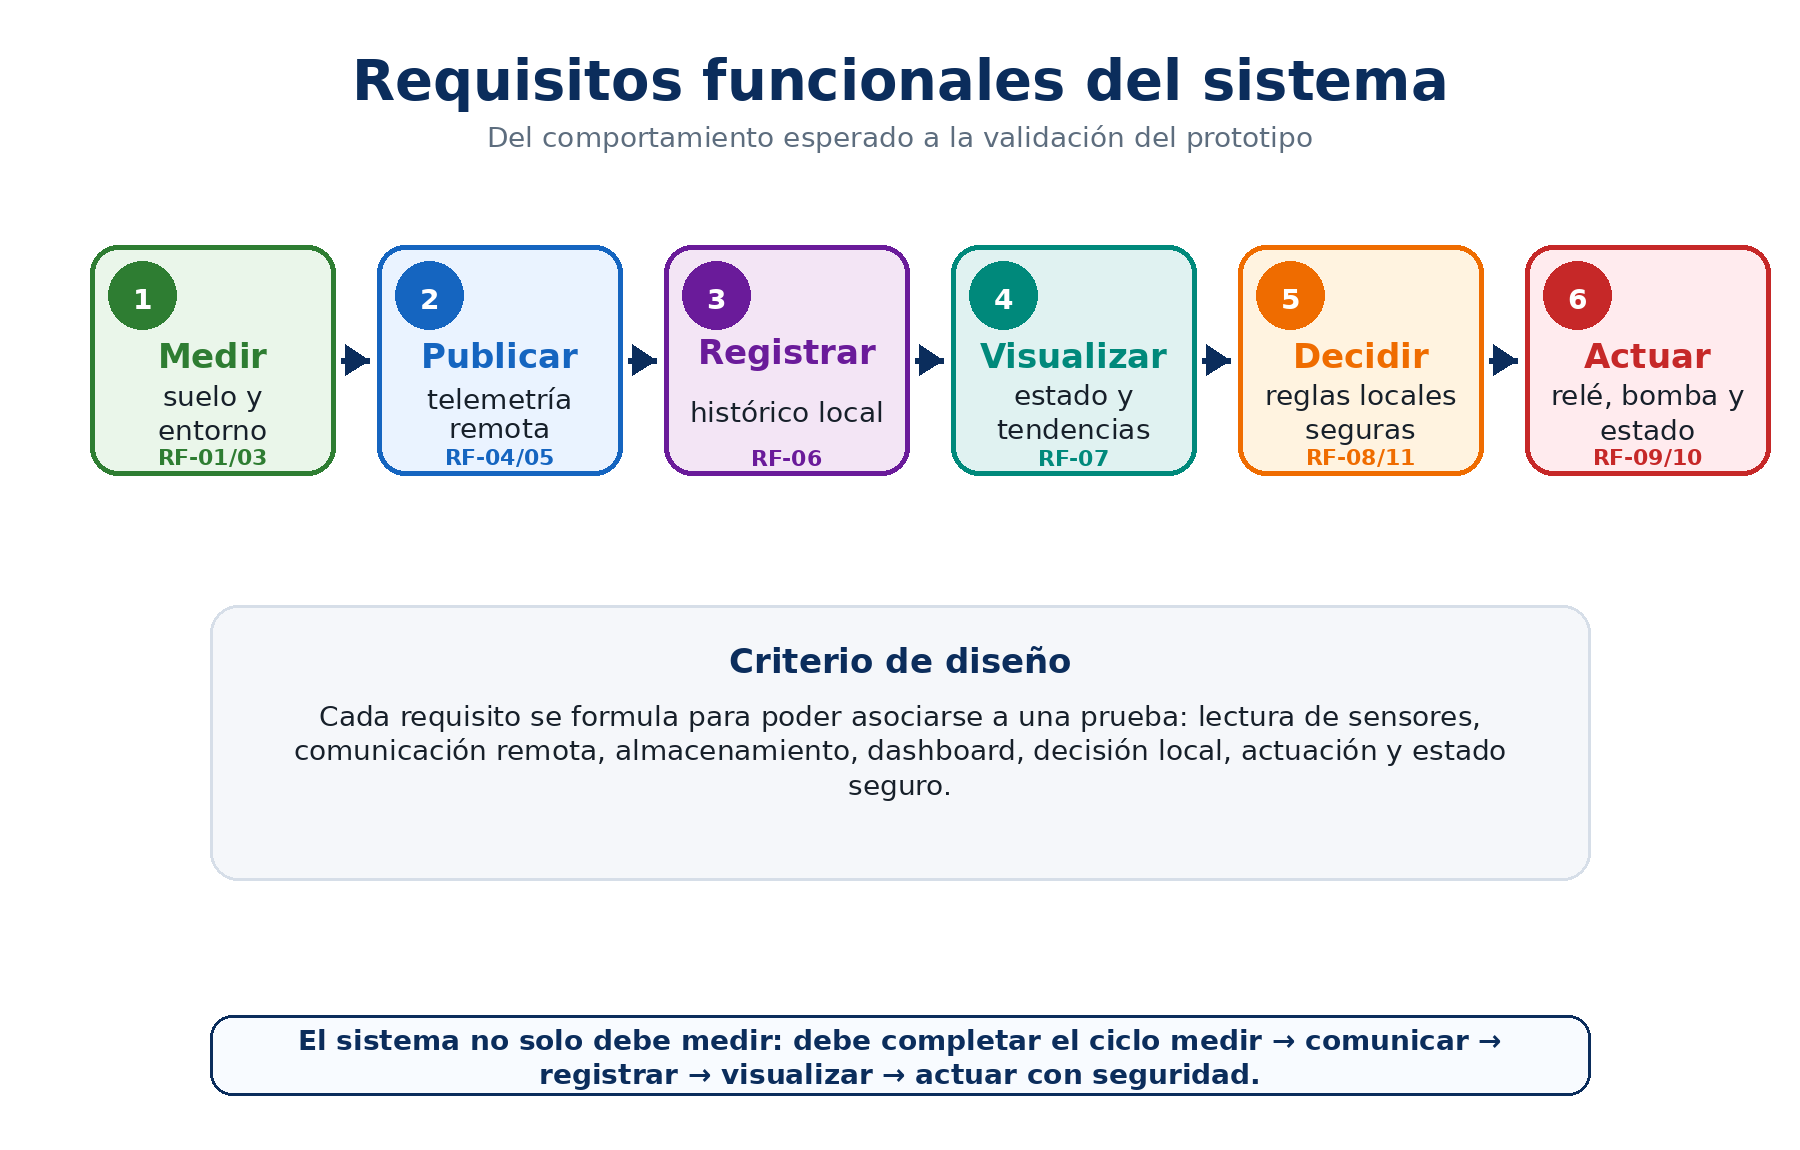
\includegraphics[width=\textwidth]{figs/figura_3_1_requisitos_funcionales.png}
    \caption{Relación entre los requisitos funcionales y el ciclo completo de funcionamiento del sistema. TierraViva debe medir, publicar telemetría, registrar histórico, visualizar el estado, decidir localmente y actuar sobre el riego de forma segura.}
    \label{fig:cap3_requisitos_funcionales}
\end{figure}

En la Tabla~\ref{cuadro:requisitos_funcionales} se recogen los principales requisitos funcionales considerados para el diseño del prototipo.

\begin{table}[H]
\centering
\small
\setlength{\tabcolsep}{4pt}
\renewcommand{\arraystretch}{1.15}
\rowcolors{2}{TableRowSoft}{white}

\makebox[\textwidth][c]{%
\hspace*{-0.7cm}%
\begin{tabular}{|
>{\raggedright\arraybackslash}p{0.06\textwidth}|
>{\raggedright\arraybackslash}p{0.22\textwidth}|
>{\raggedright\arraybackslash}p{0.52\textwidth}|
>{\raggedright\arraybackslash}p{0.24\textwidth}|}
\hline
\rowcolor{URJCRed}
\TVHead{Código} & \TVHead{Requisito} & \TVHead{Descripción} & \TVHead{Validación prevista} \\
\hline
RF-01 & Medición de humedad del suelo & El sistema debe obtener lecturas periódicas de la humedad del sustrato en la zona monitorizada. & Prueba con sensor capacitivo de humedad del suelo. \\
\hline
RF-02 & Medición ambiental & El sistema debe medir variables ambientales relevantes, incluyendo temperatura, humedad relativa y presión atmosférica. & Prueba con sensor ambiental. \\
\hline
RF-03 & Medición de luminosidad & El sistema debe registrar la luminosidad o nivel de luz ambiente para contextualizar las condiciones del entorno. & Prueba con variación de luz. \\
\hline
RF-04 & Envío remoto de telemetría & Las estaciones de campo deben enviar sus medidas a una plataforma remota para que puedan ser consultadas posteriormente. & Prueba de comunicación remota y recepción en plataforma cloud. \\
\hline
RF-05 & Identificación de estación & Cada lectura debe poder asociarse a la estación de origen, permitiendo distinguir los datos de distintas zonas o nodos. & Comprobación de registros diferenciados por estación. \\
\hline
RF-06 & Almacenamiento histórico & El sistema debe registrar las lecturas recibidas para conservar un histórico de funcionamiento. & Verificación de inserciones en SQLite. \\
\hline
RF-07 & Visualización del estado & El sistema debe ofrecer una interfaz de consulta que permita ver las últimas lecturas y el estado general del prototipo. & Prueba de dashboard web en navegador. \\
\hline
RF-08 & Decisión local de riego & Cada estación debe evaluar localmente si las condiciones medidas justifican una actuación sobre el riego. & Prueba de regla local de humedad, cooldown y estado seguro. \\
\hline
RF-09 & Actuación local sobre el riego & La estación debe accionar físicamente el sistema de riego mediante relé y bomba de agua durante un tiempo limitado por firmware. & Prueba controlada con relé y bomba/carga de prueba. \\
\hline
RF-10 & Publicación de estado de actuación & La estación debe publicar el estado del relé, el evento de sistema y un código auxiliar de diagnóstico que permitan conocer si se ha producido una actuación, una situación de reposo, un error, un estado seguro o un bloqueo por cooldown. & Verificación de \texttt{relay\_state}, \texttt{system\_event} y \texttt{debug\_code} en ThingSpeak. \\
\hline
RF-11 & Seguridad de funcionamiento & El sistema debe desactivar o mantener apagada la bomba ante error de sensor, lectura inválida, fallo de comunicación, reinicio, cooldown activo o tiempo máximo excedido. & Pruebas de modo seguro, reinicio y límites de actuación. \\
\hline
\end{tabular}%
}

\caption{Requisitos funcionales del sistema TierraViva}
\label{cuadro:requisitos_funcionales}
\end{table}

Los requisitos funcionales se agrupan en cuatro bloques. Los requisitos RF-01 a RF-03 cubren la adquisición de información en campo mediante sensores de suelo y ambiente. Los requisitos RF-04 a RF-07 definen el flujo de datos hacia la plataforma intermedia, el almacenamiento histórico y la visualización. Por último, RF-08, RF-09 y RF-10 incorporan la decisión local de riego, la actuación física y la publicación del estado operativo de cada estación.

El requisito RF-11 se ha incluido de forma explícita porque TierraViva no se limita a monitorizar variables, sino que actúa sobre una bomba de agua. Por ello, el sistema debe adoptar un comportamiento conservador ante lecturas inválidas, reinicios, fallos de comunicación o estados no verificables.

La relación completa entre requisitos, pruebas y evidencias de validación se desarrolla en el Anexo~\ref{anexo:trazabilidad_requisitos_pruebas}. De este modo, el cuerpo principal conserva la definición del sistema y los anexos recogen la comprobación detallada.

\section{Requisitos no funcionales}
\label{sec:requisitos_no_funcionales}

Los requisitos no funcionales describen las condiciones de calidad que debe cumplir el sistema, más allá de las funciones concretas indicadas en el apartado anterior. En TierraViva estos requisitos son especialmente importantes porque el proyecto no consiste únicamente en que cada bloque funcione de forma aislada, sino en que el conjunto pueda integrarse, probarse, ampliarse y defenderse como un prototipo de ingeniería.

El sistema debe mantener un equilibrio entre ambición técnica y viabilidad. No se pretende desarrollar un producto industrial cerrado, pero sí una solución suficientemente robusta, ordenada y reproducible como para demostrar el funcionamiento completo de la arquitectura propuesta. La Tabla~\ref{cuadro:requisitos_no_funcionales} resume los principales requisitos no funcionales considerados.

\begin{figure}[H]
    \centering
    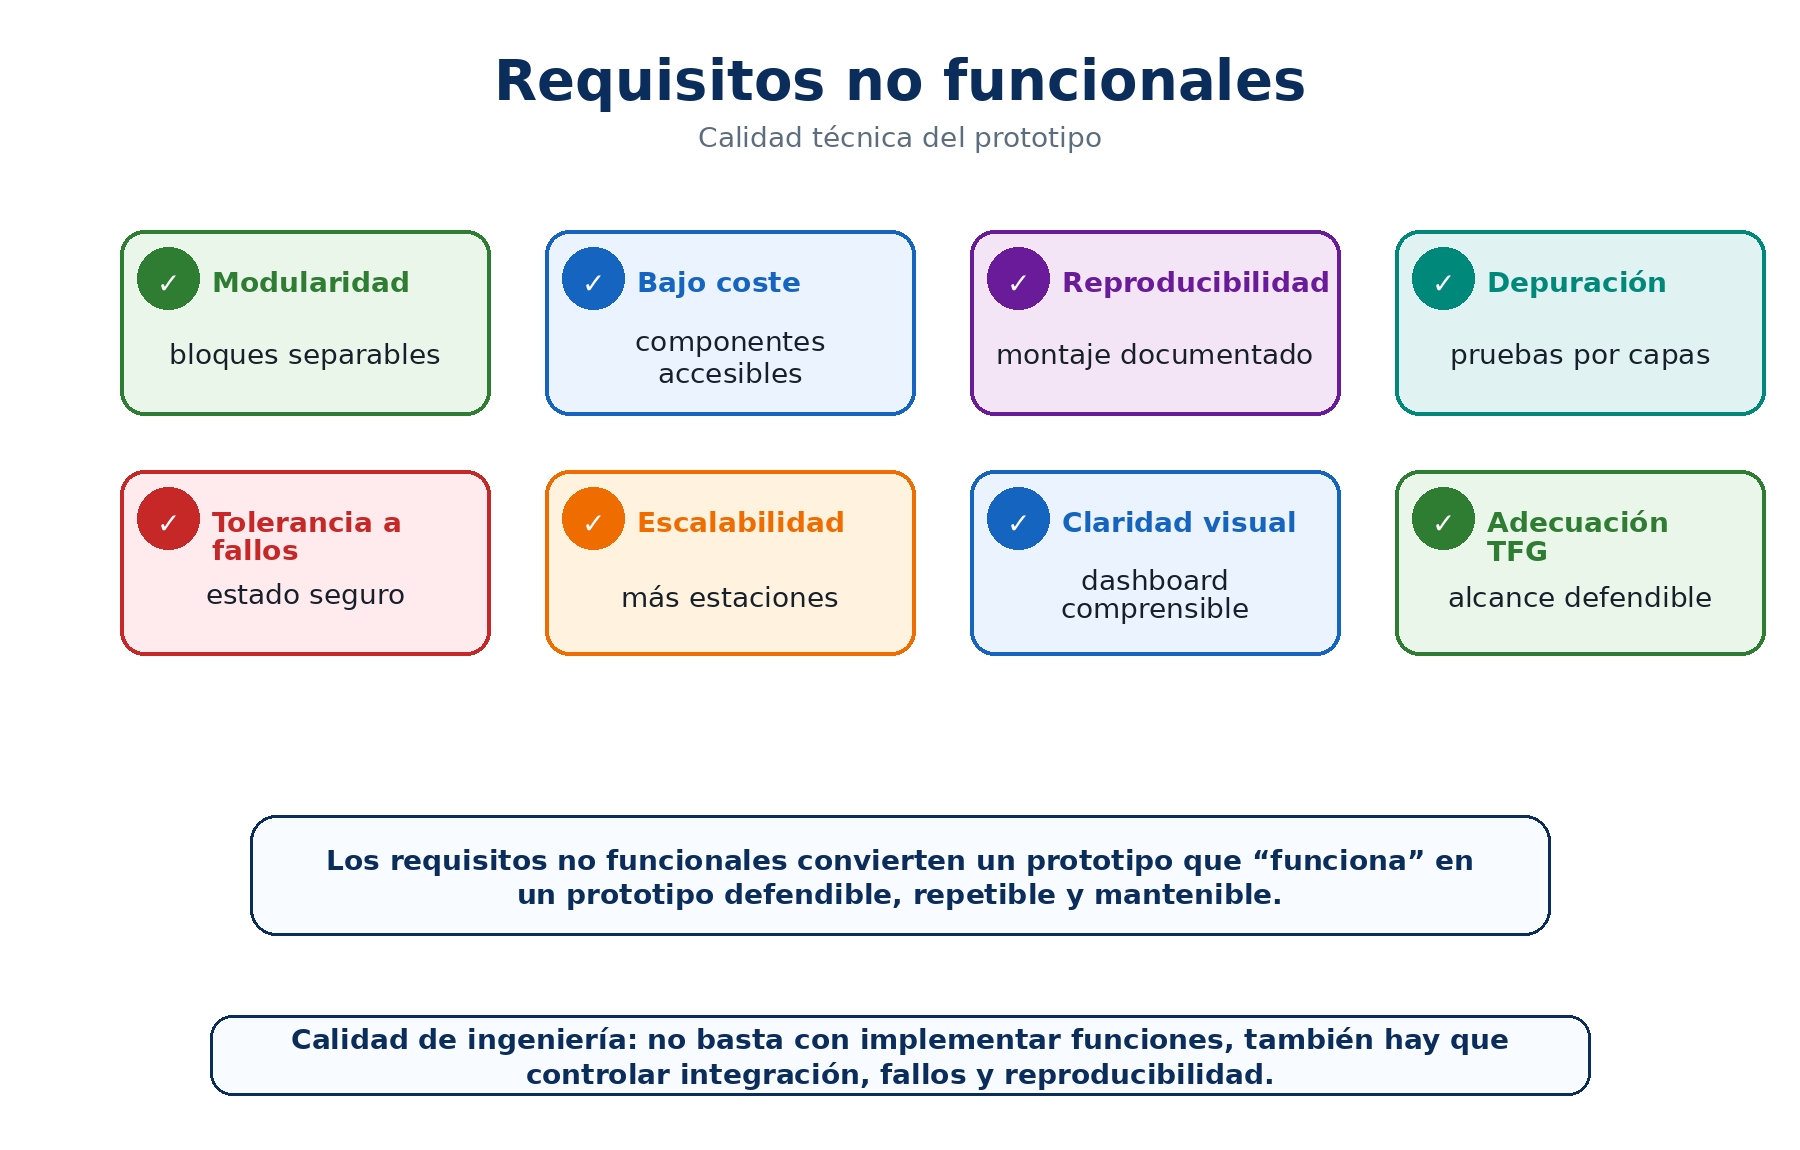
\includegraphics[width=\textwidth]{figs/figura_3_2_requisitos_no_funcionales.png}
    \caption{Requisitos no funcionales considerados en el diseño del prototipo. Estos criterios permiten evaluar la calidad técnica del sistema más allá de las funciones implementadas.}
    \label{fig:cap3_requisitos_no_funcionales}
\end{figure}

\begin{table}[H]
\begin{center}
\small
\renewcommand{\arraystretch}{1.15}
\rowcolors{2}{TableRowSoft}{white}

\begin{tabular}{|p{0.13\textwidth}|p{0.25\textwidth}|p{0.50\textwidth}|}
\hline
\rowcolor{URJCRed}
\TVHead{Código} & \TVHead{Requisito} & \TVHead{Descripción} \\
\hline
RNF-01 & Modularidad & El sistema debe organizarse en bloques diferenciados: estación de campo autónoma, comunicación, almacenamiento, supervisión, visualización y actuación local. \\
\hline
RNF-02 & Bajo coste & Los componentes seleccionados deben ser asumibles para un prototipo académico, evitando soluciones industriales de coste elevado cuando no sean necesarias. \\
\hline
RNF-03 & Reproducibilidad & El montaje, la configuración y las pruebas deben poder repetirse a partir de la documentación generada durante el proyecto. \\
\hline
RNF-04 & Facilidad de depuración & El sistema debe permitir probar los bloques por separado, identificar errores y consultar salidas intermedias durante el desarrollo. \\
\hline
RNF-05 & Consumo razonable & El diseño debe evitar consumos innecesarios y permitir una futura alimentación autónoma, aunque la optimización energética completa no sea el objetivo principal. \\
\hline
RNF-06 & Tolerancia a fallos & El sistema debe contemplar fallos de lectura, comunicación o actuación, adoptando estados seguros cuando no sea posible garantizar un funcionamiento correcto. \\
\hline
RNF-07 & Escalabilidad & La arquitectura debe permitir incorporar más de una estación de campo sin rediseñar completamente el sistema. \\
\hline
RNF-08 & Claridad de visualización & La interfaz debe presentar la información de forma comprensible, diferenciando lecturas, estados y posibles incidencias. \\
\hline
RNF-09 & Adecuación académica & El alcance debe ser realizable dentro del tiempo y medios disponibles para el TFG, priorizando funciones verificables frente a desarrollos excesivamente complejos. \\
\hline
\end{tabular}
\caption{Requisitos no funcionales del sistema TierraViva}
\label{cuadro:requisitos_no_funcionales}
\end{center}
\end{table}

Estos requisitos no funcionales condicionan la arquitectura del proyecto. La modularidad, la reproducibilidad y la facilidad de depuración justifican la separación entre estación de campo, plataforma intermedia, Raspberry Pi, API y dashboard. Esta división permite probar cada bloque de forma independiente y reduce el riesgo de que un fallo en una capa impida validar el conjunto.

El bajo coste y la adecuación académica orientan la selección de componentes hacia módulos accesibles, documentados y suficientes para demostrar el funcionamiento del sistema. La escalabilidad se plantea de forma limitada pero necesaria: el sistema debe poder trabajar con más de una estación sin rediseñar por completo la arquitectura.

La tolerancia a fallos y el consumo razonable son especialmente relevantes por la presencia de actuación física. La estación debe mantener un comportamiento seguro ante errores de lectura, comunicación o alimentación, y el diseño debe dejar abierta la posibilidad de una alimentación autónoma en futuras versiones. El análisis ampliado de riesgos se recoge en el Anexo~\ref{anexo:gestion_riesgos}.

\section{Especificaciones temporales y operativas}
\label{sec:especificaciones_temporales_operativas}

Además de los requisitos funcionales y no funcionales, el sistema necesita definir una serie de parámetros temporales y criterios operativos que regulen su comportamiento durante el funcionamiento. En un sistema IoT de riego, estos valores son importantes porque afectan al consumo energético, a la carga de comunicaciones, a la capacidad de respuesta y, sobre todo, a la seguridad de la actuación sobre la bomba de agua.

Las especificaciones temporales no se plantean como valores rígidos e inmodificables, sino como parámetros iniciales de diseño. Durante el desarrollo y la validación del prototipo pueden ajustarse en función de los resultados obtenidos, siempre manteniendo dos criterios principales: evitar comunicaciones innecesarias y garantizar que cualquier actuación sobre el riego quede limitada en el tiempo.

\begin{figure}[H]
    \centering
    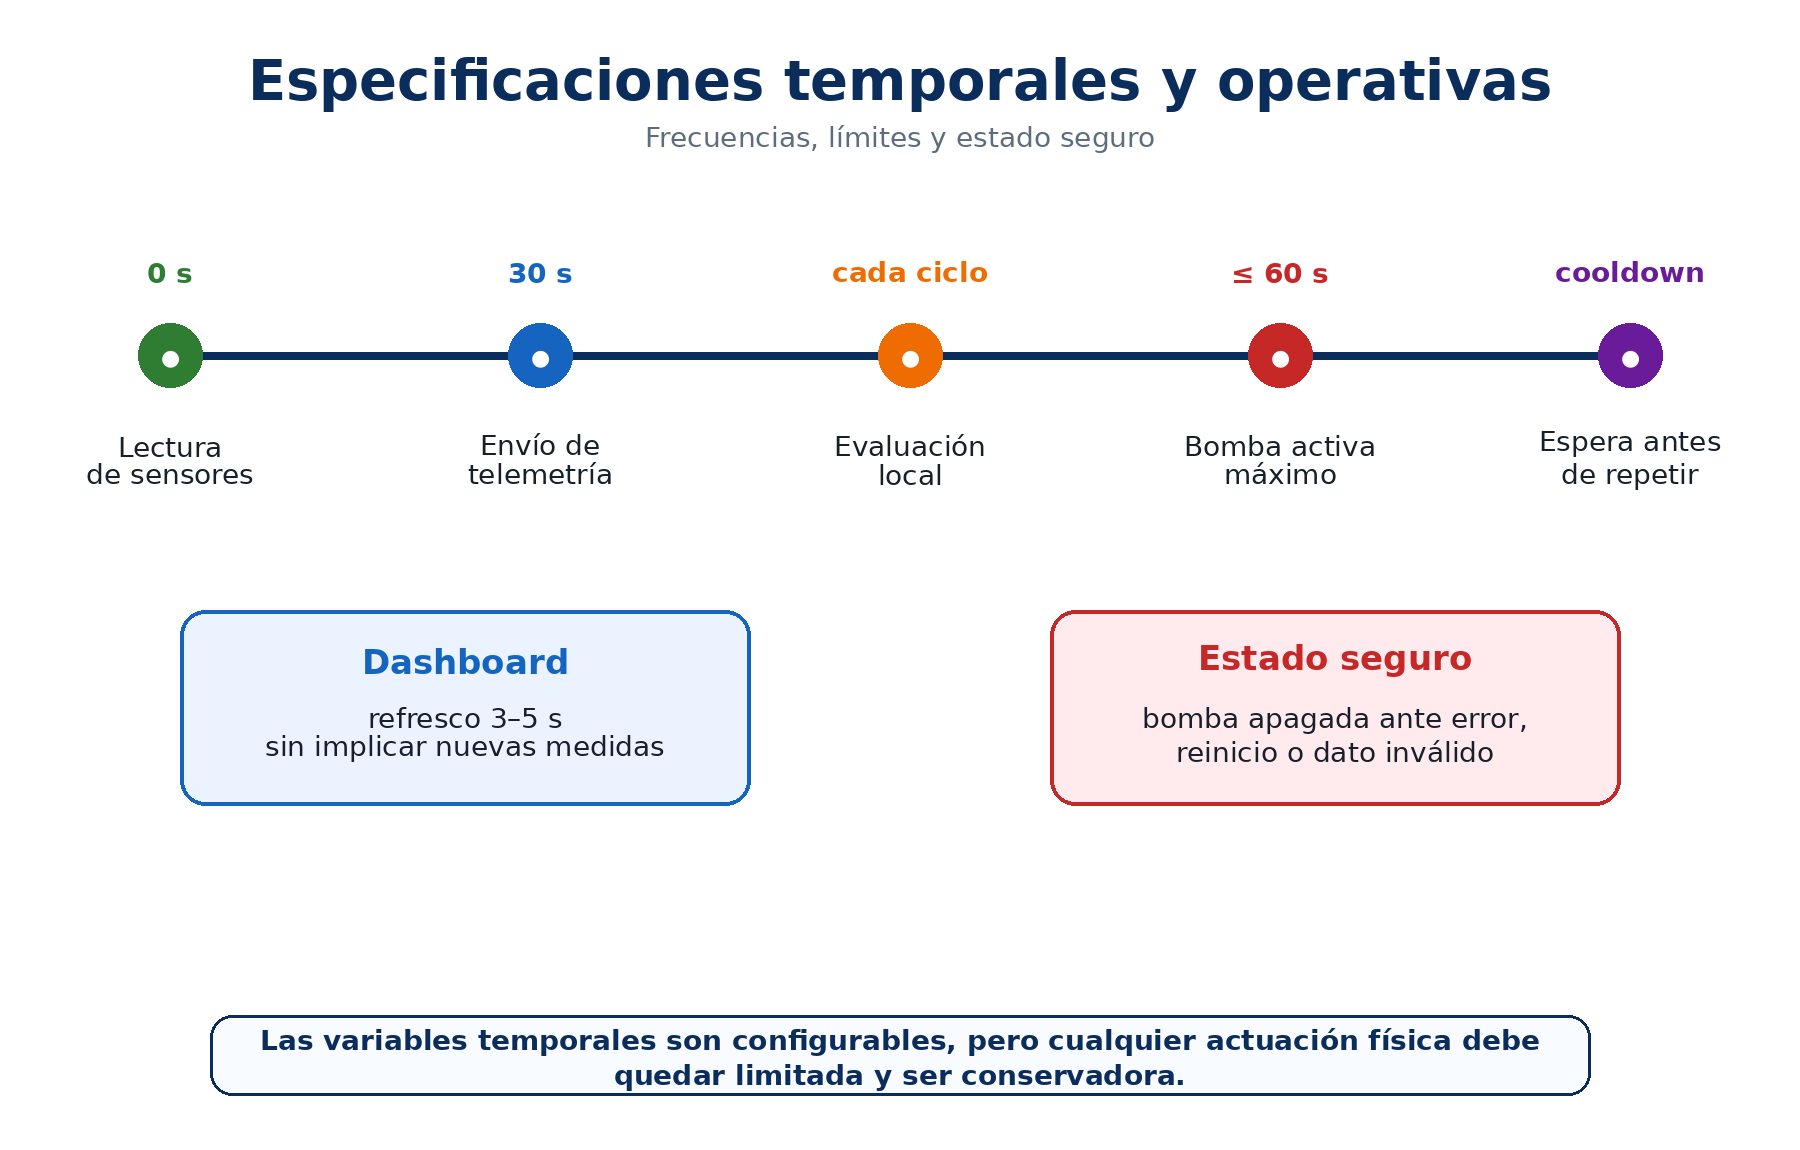
\includegraphics[width=0.85\textwidth]{figs/figura_3_3_especificaciones_temporales.png}
    \caption{Especificaciones temporales y operativas iniciales del sistema.}
    \label{fig:cap3_especificaciones_temporales}
\end{figure}

En la Tabla~\ref{cuadro:especificaciones_temporales} se recogen las principales especificaciones temporales y operativas consideradas para TierraViva.

\begin{table}[H]
\centering
\footnotesize
\renewcommand{\arraystretch}{1.15}
\rowcolors{2}{TableRowSoft}{white}

\makebox[\textwidth][c]{%
\hspace*{-0.7cm}%
\begin{tabular}{|
>{\raggedright\arraybackslash}p{0.09\textwidth}|
>{\raggedright\arraybackslash}p{0.28\textwidth}|
>{\raggedright\arraybackslash}p{0.17\textwidth}|
>{\raggedright\arraybackslash}p{0.38\textwidth}|}
\hline
\rowcolor{URJCRed}
\TVHead{Código} & \TVHead{Parámetro} & \TVHead{Valor inicial} & \TVHead{Criterio operativo} \\
\hline
ET-01 & Periodo de lectura de sensores & Configurable & Las estaciones toman medidas periódicas del entorno. Durante pruebas pueden utilizarse intervalos reducidos para acelerar la validación. \\
\hline
ET-02 & Frecuencia de envío de telemetría & Configurable & Cada estación envía sus datos de forma periódica, evitando tráfico innecesario en funcionamiento normal. \\
\hline
ET-03 & Frecuencia de actualización del dashboard & 3--5 s & La interfaz consulta el estado con mayor frecuencia que la llegada real de nuevos datos. \\
\hline
ET-04 & Intervalo de evaluación local & Configurable & Cada estación evalúa periódicamente sus lecturas y comprueba si se cumplen las condiciones locales de riego. \\
\hline
ET-05 & Tiempo máximo de bomba activa & Configurable & La activación de la bomba queda limitada por firmware para evitar riego indefinido ante errores de control. \\
\hline
ET-06 & Tiempo mínimo entre riegos & Configurable & Se aplica un periodo de espera para evitar actuaciones repetidas en poco tiempo. \\
\hline
ET-07 & Tiempo máximo sin dato reciente en supervisión & Configurable & La Raspberry Pi y el dashboard deben identificar lecturas antiguas u offline cuando no se reciben publicaciones recientes de una estación. \\
\hline
ET-08 & Estado seguro por defecto & Bomba apagada & Al arrancar, ante error de lectura, fallo de comunicación o condición no verificable, la estación mantiene desactivado el riego. \\
\hline
ET-09 & Comportamiento ante dato inválido & Ignorar y registrar & Las lecturas no válidas no deben provocar una actuación automática. \\
\hline
ET-10 & Comportamiento ante pérdida de comunicación & Bomba apagada o no actuación & La pérdida de comunicación no debe dejar la bomba activa. \\
\hline
\end{tabular}%
}

\caption{Especificaciones temporales y operativas iniciales del sistema}
\label{cuadro:especificaciones_temporales}
\end{table}

Los parámetros temporales se definen como valores configurables del firmware. Durante las pruebas pueden emplearse intervalos reducidos para acelerar la validación, mientras que en un funcionamiento más estable conviene utilizar periodos más conservadores. Lo importante desde el punto de vista de diseño no es fijar un único valor definitivo, sino garantizar ciclos controlados, detección de datos antiguos en supervisión y actuación de la bomba siempre limitada temporalmente.

La actualización del dashboard puede realizarse con mayor frecuencia que la publicación de las estaciones, pero no debe interpretarse como una nueva medida en cada refresco. La actuación física queda gobernada por el firmware de la estación, que debe mantener la bomba apagada ante lecturas inválidas, reinicios, pérdida de comunicación o estados no verificables.

\section{Metodología de trabajo}
\label{sec:metodologia_trabajo}

La metodología seguida en TierraViva se ha basado en un desarrollo incremental por bloques. En lugar de intentar construir el sistema completo desde el primer momento, se ha dividido el proyecto en fases más pequeñas, cada una orientada a validar una parte concreta de la arquitectura. Este enfoque resulta adecuado para un sistema IoT con sensores, comunicaciones, almacenamiento, visualización y actuación física, ya que permite aislar errores y reducir el riesgo de integración.

La idea principal ha sido avanzar desde pruebas controladas hacia una arquitectura cada vez más cercana al funcionamiento final. Primero se analizaron las necesidades del problema y las alternativas tecnológicas disponibles. Después se desarrollaron prototipos parciales para comprobar sensores, comunicaciones, almacenamiento y visualización. Finalmente, las distintas partes se fueron conectando hasta formar una solución de monitorización y control más completa.

Esta forma de trabajo también ha permitido documentar decisiones y cambios de enfoque. En un proyecto de este tipo, no todas las decisiones se pueden cerrar desde el principio, ya que algunas dependen de la disponibilidad real de hardware, de la facilidad de integración o de los resultados obtenidos en pruebas. Por ello, la metodología no se ha limitado a implementar una arquitectura previamente fija, sino que ha incorporado revisión, validación y corrección de decisiones durante el desarrollo.

En la Tabla~\ref{cuadro:metodologia_fases} se resumen las fases principales seguidas durante el proyecto.

\begin{table}[H]
\centering
\footnotesize
\renewcommand{\arraystretch}{1.15}
\rowcolors{2}{TableRowSoft}{white}

\makebox[\textwidth][c]{%
\hspace*{-0.7cm}%
\begin{tabular}{|
>{\raggedright\arraybackslash}p{0.07\textwidth}|
>{\raggedright\arraybackslash}p{0.24\textwidth}|
>{\raggedright\arraybackslash}p{0.68\textwidth}|}
\hline
\rowcolor{URJCRed}
\TVHead{Fase} & \TVHead{Nombre} & \TVHead{Objetivo principal} \\
\hline
1 & Análisis inicial del problema & Identificar la necesidad de monitorizar y controlar el riego en un entorno no supervisado de forma continua. \\
\hline
2 & Revisión tecnológica & Estudiar alternativas de sensorización, plataformas embebidas, comunicaciones, almacenamiento, visualización y actuación. \\
\hline
3 & Diseño conceptual de la arquitectura & Definir los bloques principales del sistema y la relación entre estaciones autónomas de campo, plataforma intermedia, sistema de supervisión y actuador. \\
\hline
4 & Prototipo local con Raspberry & Validar una primera cadena de adquisición, mensajería, almacenamiento y visualización mediante Raspberry Pi, MQTT, SQLite, FastAPI y dashboard. \\
\hline
5 & Validación de sensores & Comprobar el funcionamiento de los sensores de humedad de suelo, luminosidad y variables ambientales antes de integrarlos en una estación. \\
\hline
6 & Validación de comunicaciones & Probar la comunicación remota necesaria para publicar telemetría y estado desde las estaciones. \\
\hline
7 & Elección de plataforma cloud & Seleccionar una plataforma intermedia que permitiera publicar telemetría, consultar datos remotos y supervisar el estado de las estaciones de forma sencilla y verificable. \\
\hline
8 & Diseño de actuación local & Definir el control autónomo de la bomba de agua mediante relé, incluyendo reglas locales, tiempos máximos, cooldown y estado seguro. \\
\hline
9 & Integración de subsistemas & Conectar adquisición, comunicación, supervisión, almacenamiento, visualización, decisión local y actuación en una arquitectura coherente. \\
\hline
10 & Validación experimental & Comprobar el funcionamiento del sistema mediante pruebas parciales, pruebas de estación autónoma y pruebas de supervisión extremo a extremo. \\
\hline
11 & Documentación de incidencias y decisiones & Registrar problemas encontrados, alternativas descartadas, cambios de enfoque y criterios técnicos adoptados. \\
\hline
\end{tabular}%
}

\caption{Fases principales de la metodología de trabajo}
\label{cuadro:metodologia_fases}
\end{table}

Las primeras fases permitieron transformar la necesidad inicial en requisitos técnicos y revisar las alternativas de sensorización, comunicaciones, plataformas embebidas, almacenamiento y visualización. A partir de esa revisión se definió una arquitectura por bloques, con estaciones autónomas de campo, plataforma intermedia, sistema de supervisión y actuación local.

El prototipo local previo con Raspberry Pi permitió validar una primera cadena de adquisición, almacenamiento, API y dashboard antes de adoptar la arquitectura final con LTE y ThingSpeak. Posteriormente se validaron sensores, comunicaciones y actuación por separado, evitando mezclar problemas de cableado, alimentación, módem, backend o lógica de riego en una única fase de integración.

La integración final conectó adquisición, publicación de telemetría, almacenamiento local, visualización, decisión local y actuación sobre el relé. Durante este proceso se documentaron incidencias, alternativas descartadas y cambios de enfoque, especialmente la separación entre supervisión y control local. Esta decisión trasladó la lógica crítica de riego al firmware de cada estación y dejó la Raspberry Pi como sistema de consulta, histórico y visualización.

\section{Arquitectura general planteada}
\label{sec:arquitectura_general_planteada}

A partir de los requisitos definidos en los apartados anteriores, la arquitectura general de TierraViva se plantea como un sistema IoT distribuido, formado por estaciones autónomas de campo, una plataforma intermedia de comunicación y un sistema de supervisión basado en Raspberry Pi. El objetivo de esta arquitectura es separar claramente la adquisición de datos, la decisión local, la actuación física, la publicación de telemetría, el almacenamiento histórico y la visualización.

La arquitectura se ha diseñado teniendo en cuenta una restricción importante: las estaciones de campo no están conectadas físicamente a la Raspberry Pi. Por tanto, no se puede asumir una comunicación directa mediante USB, puerto serie o red local entre ambos extremos. Las estaciones deben poder enviar datos de forma remota mediante el módulo LTE, y la Raspberry debe consultar esa información desde la plataforma intermedia. Esto condiciona el diseño completo del sistema y evita que el riego dependa de una conexión local o de una orden enviada desde la Raspberry.

En términos generales, el sistema se divide en cuatro bloques principales:

\begin{itemize}
    \item \textbf{Estaciones autónomas de campo}: encargadas de medir las variables del entorno, evaluar reglas locales de riego, accionar la bomba mediante relé y publicar telemetría y estado.
    \item \textbf{Capa de comunicaciones y plataforma intermedia}: responsable de recibir los datos publicados por las estaciones y hacerlos accesibles para consulta remota.
    \item \textbf{Sistema de supervisión}: implementado sobre Raspberry Pi, encargado de consultar datos, almacenarlos, exponer una API y servir el dashboard.
    \item \textbf{Interfaz de usuario}: orientada a visualizar el estado del sistema, revisar el histórico y supervisar las actuaciones realizadas por las estaciones.
\end{itemize}

La Figura~\ref{fig:arquitectura_general_tierraviva} muestra una visión general de la arquitectura planteada.

\begin{figure}[H]
  \hspace{-0.5cm}\centerline{\resizebox{1.2\textwidth}{!}{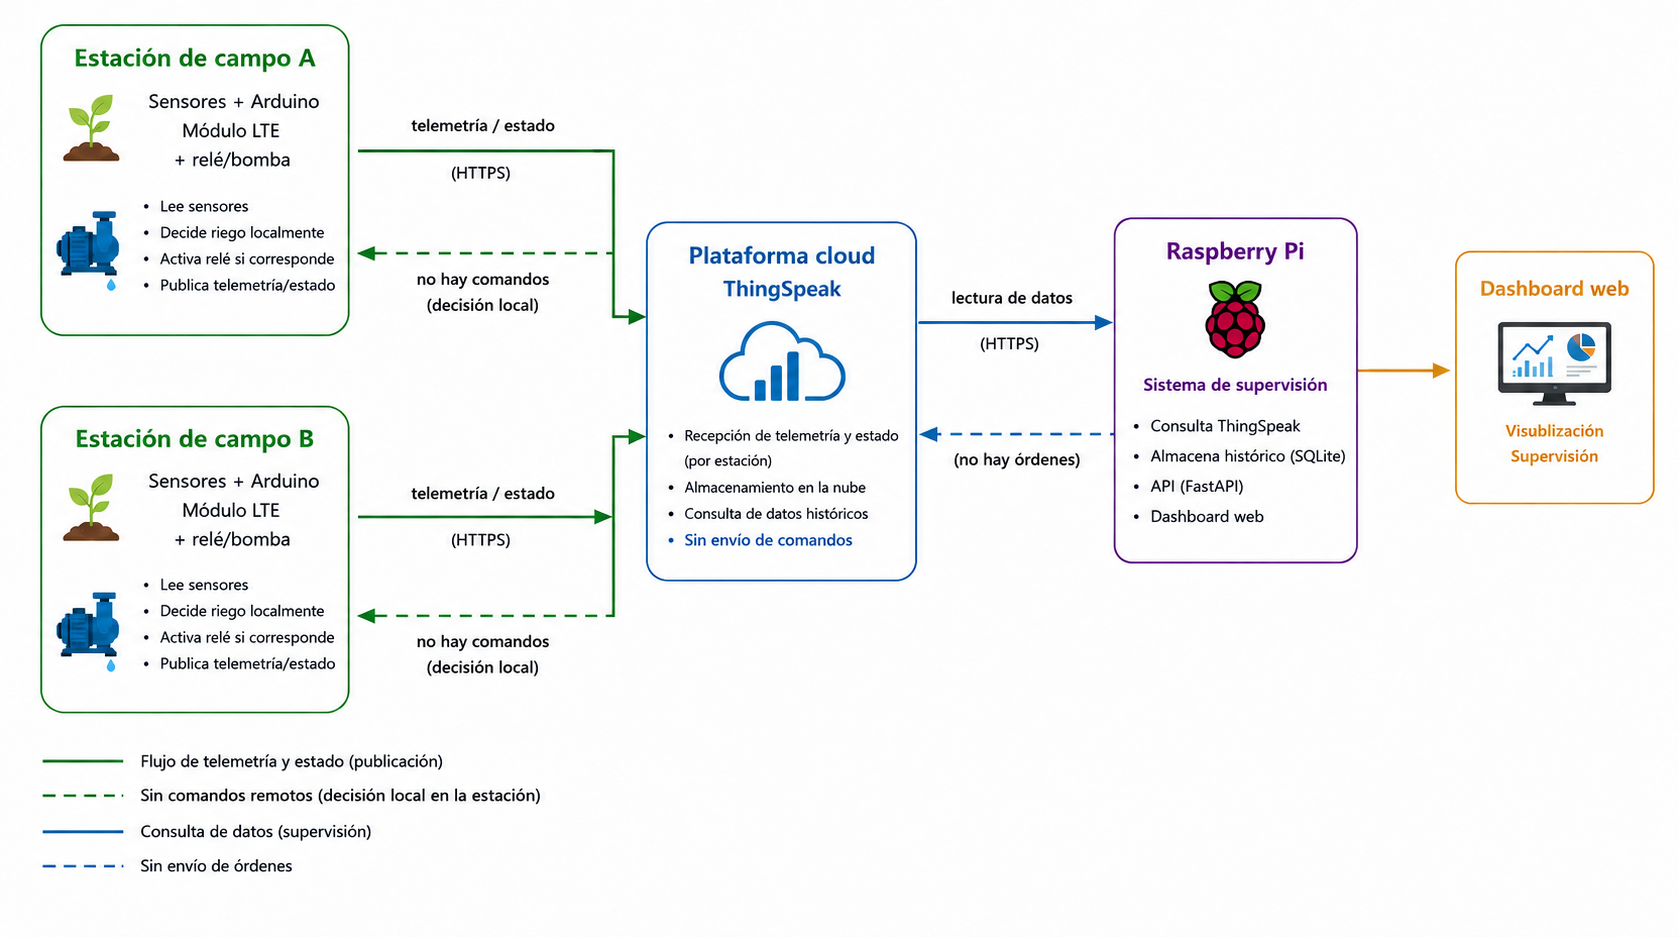
\includegraphics{figs/arquitecturaTierraViva.png}}}
  \caption{Arquitectura general planteada para TierraViva.}
\label{fig:arquitectura_general_tierraviva}
\end{figure}

La división de responsabilidades es el punto central de esta arquitectura. Las estaciones de campo interactúan con el entorno físico, toman la decisión local de riego y publican telemetría. ThingSpeak actúa como plataforma intermedia de comunicación. La Raspberry Pi consulta los datos, mantiene el histórico, expone la API y sirve el dashboard, sin convertirse en el elemento responsable de decidir la activación de la bomba.

El detalle de la arquitectura final, incluyendo canales de ThingSpeak, flujo de telemetría y papel de cada bloque, se desarrolla en el Capítulo~\ref{cap:capitulo4}. Los flujos visuales de funcionamiento se recogen en el Anexo~\ref{anexo:diagramas_flujo_funcionamiento}.

\section{Elección de variables y sensores}
\label{sec:eleccion_variables_sensores}

La selección de variables medidas se ha realizado teniendo en cuenta el papel que deben cumplir dentro del prototipo: monitorizar el estado de una zona de cultivo y aportar información suficiente para alimentar la decisión local de riego en cada estación. No se pretende medir todos los parámetros agronómicos posibles, sino elegir un conjunto reducido de variables que permita validar el comportamiento del prototipo de forma razonable, reproducible y coherente con el alcance del TFG.

En TierraViva se combinan variables del suelo y variables ambientales. La humedad del suelo se considera la variable principal para la decisión local de riego, ya que aporta información directa sobre la disponibilidad de agua en el sustrato. Las variables ambientales, como temperatura, humedad relativa, presión atmosférica y luminosidad, no sustituyen a la humedad del suelo, pero ayudan a interpretar el contexto en el que evoluciona la zona monitorizada. Esta combinación es habitual en sistemas de agricultura de precisión basados en sensores, donde el interés no está solo en una lectura aislada, sino en la observación conjunta del entorno \cite{soussi2024smart}.

\begin{figure}[H]
    \centering
    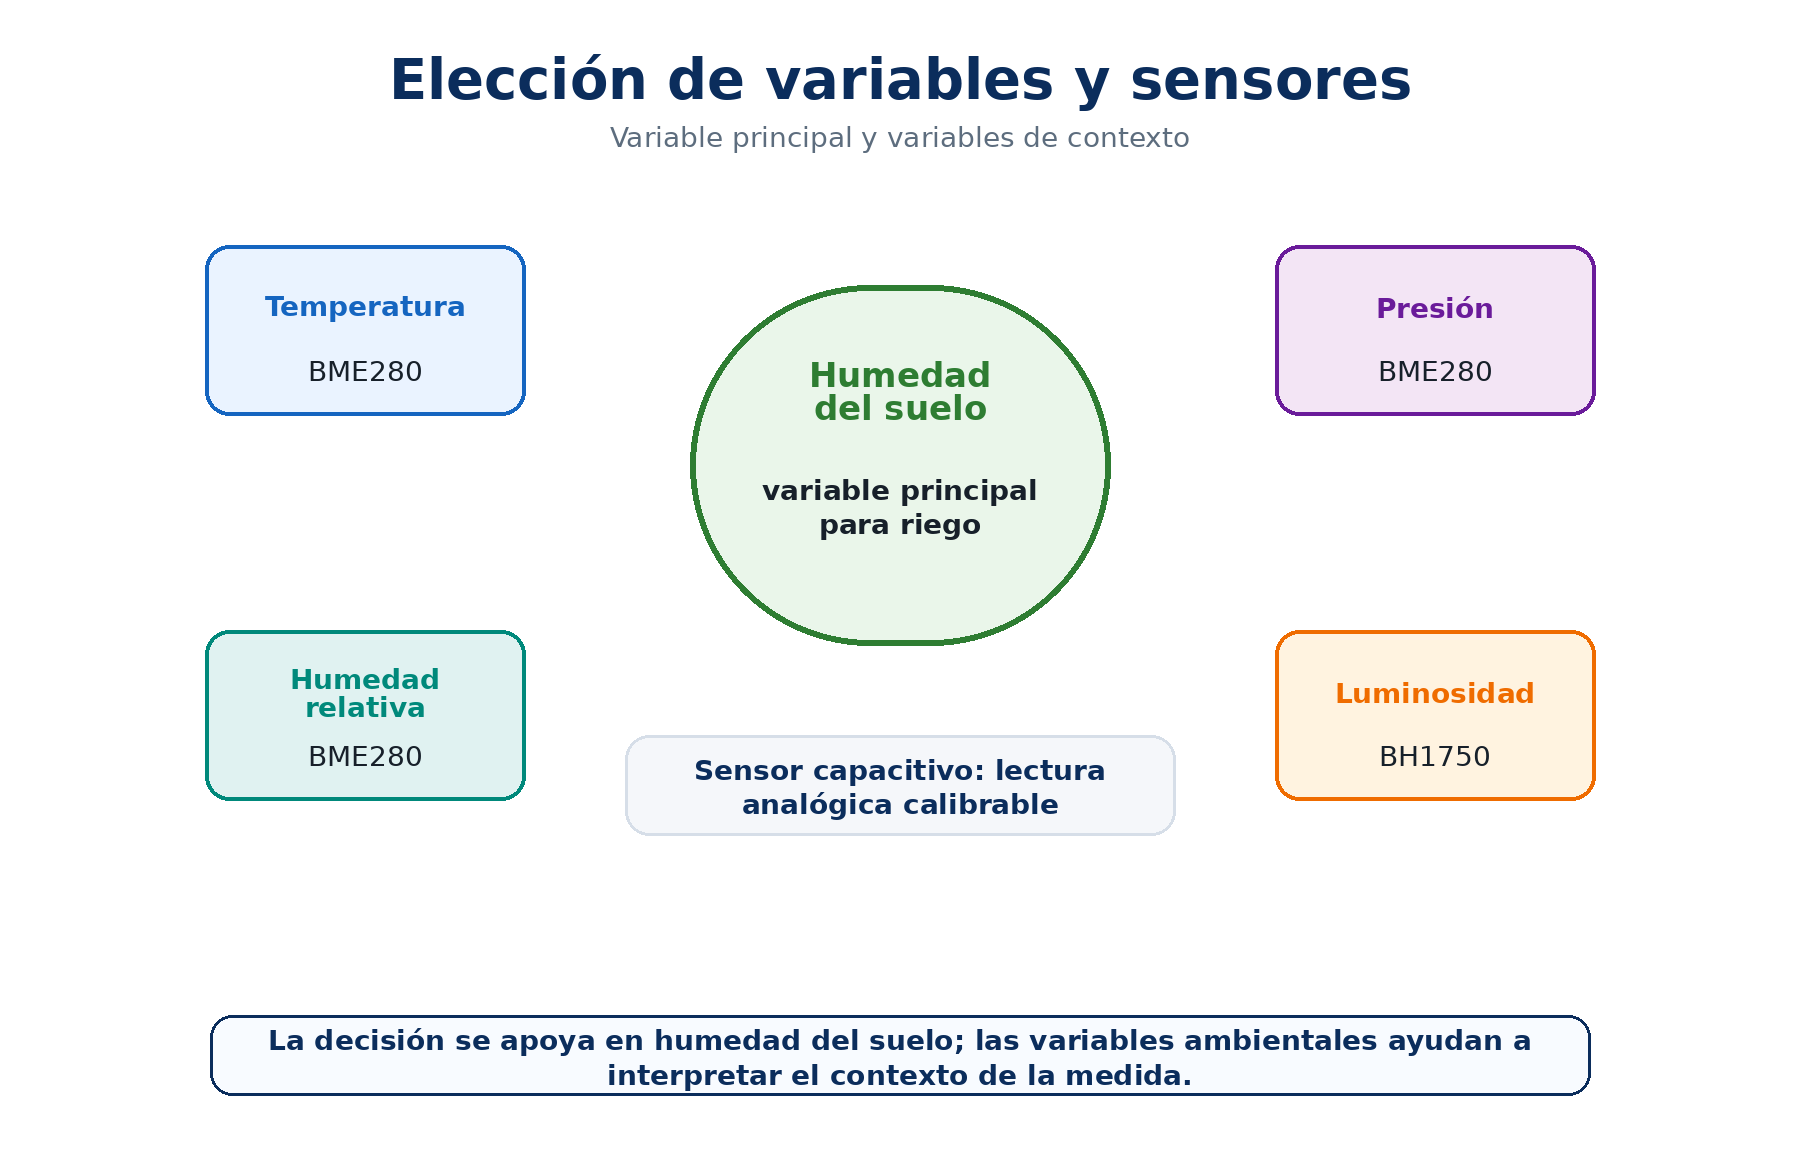
\includegraphics[width=\textwidth]{figs/figura_3_6_variables_sensores.png}
    \caption{Variables seleccionadas para la monitorización de TierraViva. La humedad del suelo se utiliza como variable principal para la decisión local de riego, mientras que temperatura, humedad relativa, presión y luminosidad aportan contexto ambiental.}
    \label{fig:cap3_variables_sensores}
\end{figure}

La Figura~\ref{fig:cap3_variables_sensores} resume las variables seleccionadas. La humedad del suelo actúa como variable principal de decisión, mientras que temperatura, humedad relativa, presión atmosférica y luminosidad aportan contexto ambiental. La correspondencia entre sensores y magnitudes medidas se recoge en la Tabla~\ref{cuadro:sensores_seleccionados}.

La humedad del suelo se ha seleccionado como variable principal porque es la medida más directamente relacionada con la necesidad de riego. En el prototipo se utiliza un sensor capacitivo de humedad de suelo V1.2, cuya salida analógica permite integrarlo de forma sencilla con Arduino. Frente a sensores resistivos, este tipo de sensor reduce los problemas de degradación por contacto con humedad, aunque requiere calibración para interpretar sus valores como porcentaje útil de humedad \cite{azdelivery_soil_v12}.

Las variables ambientales se incorporan como información de contexto. La temperatura, la humedad relativa y la presión se obtienen mediante el BME280, que integra las tres magnitudes en un único módulo digital con comunicación I2C \cite{bosch_bme280_datasheet}. La luminosidad se mide mediante el BH1750/GY-302, que proporciona valores en lux y permite interpretar la exposición solar de la zona monitorizada \cite{rohm_bh1750_datasheet}.

\begin{table}[H]
\begin{center}
\small
\renewcommand{\arraystretch}{1.15}
\rowcolors{2}{TableRowSoft}{white}

\begin{tabular}{|p{0.26\textwidth}|p{0.26\textwidth}|p{0.36\textwidth}|}
\hline
\rowcolor{URJCRed}
\TVHead{Sensor} & \TVHead{Variable medida} & \TVHead{Justificación de elección} \\
\hline
Sensor capacitivo de humedad de suelo V1.2 & Humedad del sustrato mediante lectura analógica. & Variable principal para riego; bajo coste; integración sencilla con Arduino; menor corrosión que sensores resistivos. \\
\hline
BME280 & Temperatura, humedad relativa y presión atmosférica. & Integra tres variables ambientales en un único módulo digital; reduce cableado; comunicación I2C. \\
\hline
BH1750 / GY-302 & Luminosidad ambiente en lux. & Proporciona medida digital de luz; comparte bus I2C; facilita interpretar exposición solar. \\
\hline
\end{tabular}
\caption{Sensores seleccionados para las estaciones de campo}
\label{cuadro:sensores_seleccionados}
\end{center}
\end{table}

La elección de estos sensores responde a criterios prácticos: bajo coste, disponibilidad, documentación accesible, compatibilidad con Arduino y posibilidad de validar el sistema sin instrumentación industrial. El detalle de componentes se recoge en el Anexo~\ref{anexo:materiales}; el conexionado eléctrico, en el Anexo~\ref{anexo:esquemas_electricos}; y la estrategia de validación, en los Anexos~\ref{anexo:plan_pruebas} y \ref{anexo:trazabilidad_requisitos_pruebas}.

En conjunto, la combinación seleccionada cubre una variable principal de decisión, la humedad del suelo, y varias variables ambientales de contexto. Sensores más avanzados, como caudal, nivel de depósito, conductividad eléctrica o pH, quedan como posibles ampliaciones futuras.

\section{Elección de plataforma de control local y supervisión}
\label{sec:eleccion_plataformas_control}

La arquitectura de TierraViva separa claramente dos niveles funcionales. Por un lado, las estaciones de campo necesitan una plataforma sencilla y cercana al hardware, capaz de leer sensores, comunicarse con el módulo LTE, aplicar reglas locales de riego y controlar el relé de la bomba. Por otro lado, el sistema necesita una plataforma con mayor capacidad software para consultar datos, almacenarlos, exponer una API y servir el dashboard web. Esta segunda plataforma no actúa como cerebro del riego, sino como sistema de supervisión e histórico. Esta diferencia de funciones justifica el uso combinado de Arduino UNO y Raspberry Pi 5, en lugar de concentrar todo el sistema en una única plataforma.

\begin{figure}[H]
    \centering
    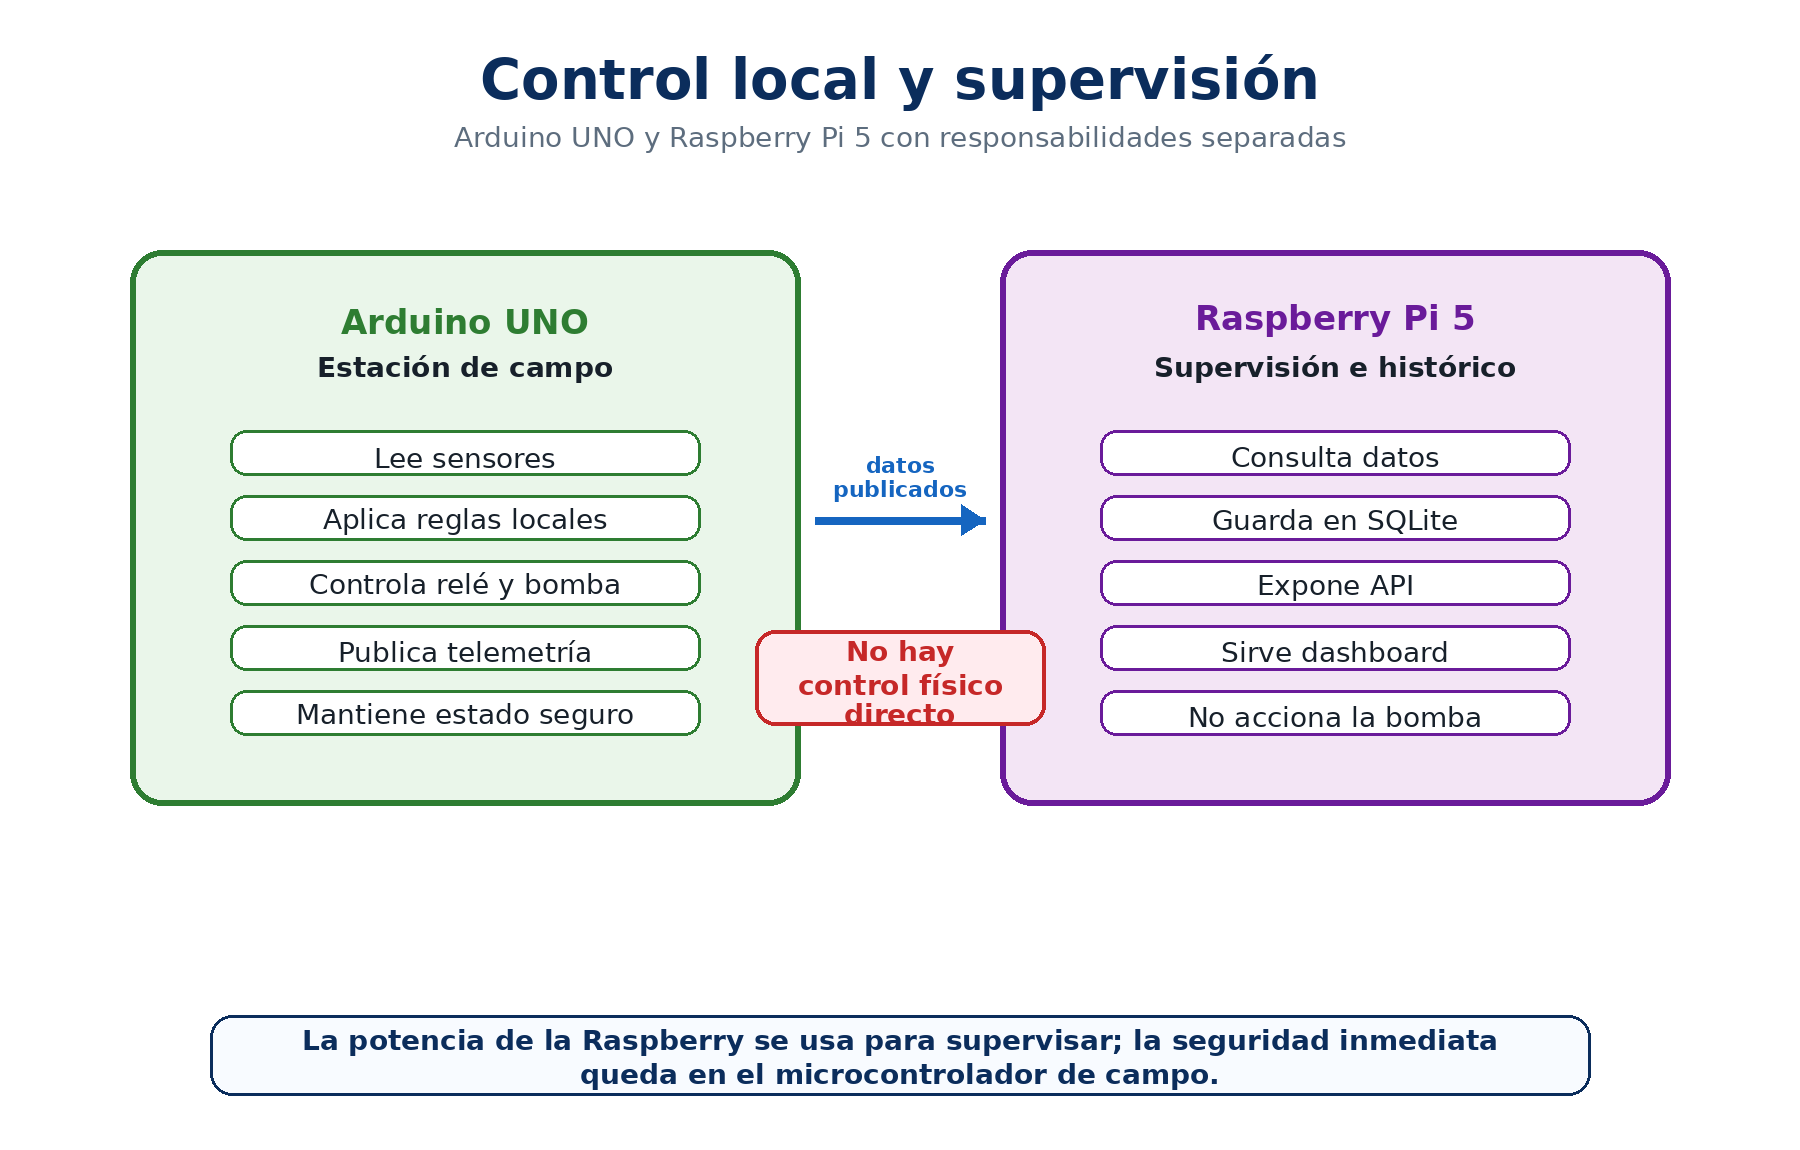
\includegraphics[width=\textwidth]{figs/figura_3_7_plataformas_control_supervision.png}
    \caption{Separación de responsabilidades entre Arduino UNO y Raspberry Pi 5.}
    \label{fig:cap3_plataformas_control_supervision}
\end{figure}

Arduino UNO se ha seleccionado como plataforma principal de las estaciones de campo porque ofrece una integración directa con sensores, bus I2C, entrada analógica, comunicación serie con el módem LTE y control digital del relé. Sus prestaciones son limitadas frente a plataformas más modernas, pero suficientes para las tareas previstas en el nodo de campo: medir, aplicar reglas locales, comunicarse y actuar sobre la bomba \cite{arduino_uno_rev3_specs}.

La Raspberry Pi 5 se utiliza como sistema de supervisión, no como controlador físico del riego. Su mayor capacidad permite ejecutar procesos software, mantener una base de datos local, servir una API y alojar el dashboard web \cite{raspberry_pi5_product_brief}. Esta separación evita concentrar en un único dispositivo tareas muy distintas y permite que la estación mantenga un comportamiento seguro aunque la Raspberry no esté disponible.

La Tabla~\ref{cuadro:arduino_raspberry_tierraviva} resume esta división de responsabilidades.

\begin{table}[H]
\begin{center}
\small
\renewcommand{\arraystretch}{1.15}
\rowcolors{2}{TableRowSoft}{white}

\begin{tabular}{|p{0.24\textwidth}|p{0.32\textwidth}|p{0.32\textwidth}|}
\hline
\rowcolor{URJCRed}
\TVHead{Aspecto} & \TVHead{Arduino UNO} & \TVHead{Raspberry Pi 5} \\
\hline
Rol en TierraViva & Controlador local autónomo de estación de campo. & Sistema de supervisión, almacenamiento y visualización. \\
\hline
Relación con sensores & Lectura directa de sensores analógicos y digitales. & No lee sensores directamente en la arquitectura final. \\
\hline
Actuación & Decisión local y control del relé asociado a la bomba. & No participa en la actuación física ni genera órdenes de riego. \\
\hline
Capacidad software & Firmware sencillo y tareas embebidas. & Sistema operativo, API, base de datos y dashboard. \\
\hline
Consumo y arranque & Menor consumo y arranque inmediato. & Mayor consumo y arranque dependiente del sistema operativo. \\
\hline
Adecuación principal & Nodo de campo sencillo y robusto. & Procesamiento, histórico y supervisión. \\
\hline
\end{tabular}
\caption{Comparación funcional entre Arduino UNO y Raspberry Pi 5 en TierraViva}
\label{cuadro:arduino_raspberry_tierraviva}
\end{center}
\end{table}

Durante el diseño también se consideraron alternativas como ESP32 o STM32. ESP32 habría aportado mayor potencia y conectividad integrada, pero en TierraViva la comunicación remota se resuelve mediante un módem LTE externo. STM32 ofrece más prestaciones, aunque aumenta la complejidad de configuración y depuración. Para el alcance del TFG, la combinación Arduino UNO y Raspberry Pi 5 mantiene un equilibrio adecuado entre sencillez, coste, capacidad técnica y reproducibilidad.

\section{Selección de solución de comunicaciones para estaciones remotas}
\label{sec:seleccion_comunicaciones_remotas}

La comunicación entre las estaciones de campo y el sistema de supervisión es una decisión crítica en TierraViva. Las estaciones no se consideran conectadas físicamente a la Raspberry Pi, por lo que la telemetría debe enviarse de forma remota desde la parcela o zona de cultivo. La solución elegida debía funcionar sin depender de una red WiFi local, permitir integración con una plataforma cloud y ser verificable dentro del alcance temporal del TFG.

Durante el diseño se valoraron principalmente dos enfoques: LoRa/LoRaWAN y conectividad móvil LTE. LoRa resulta especialmente atractivo en IoT agrícola por su largo alcance, bajo consumo y adecuación a mensajes pequeños \cite{semtech2015lora_modulation,augustin2016lora}. LoRaWAN añade una arquitectura de red con dispositivos finales, pasarelas y servidores de red \cite{lora_alliance_104}. Sin embargo, esta opción habría requerido resolver infraestructura adicional, selección de módulos, compatibilidad de banda, alimentación, niveles lógicos y configuración de red, desplazando una parte importante del esfuerzo hacia la propia comunicación.

LTE con el módulo A7670E-LASA se eligió como alternativa más adecuada para validar el sistema completo. Esta opción permite que cada estación publique datos directamente en Internet mediante red móvil y peticiones HTTP, sin desplegar gateway propio. A cambio, introduce dependencia de cobertura móvil, tarjeta SIM, consumo energético superior y una alimentación más exigente para el módem.

\begin{table}[H]
\begin{center}
\small
\renewcommand{\arraystretch}{1.15}
\rowcolors{2}{TableRowSoft}{white}

\begin{tabular}{|p{0.24\textwidth}|p{0.30\textwidth}|p{0.34\textwidth}|}
\hline
\rowcolor{URJCRed}
\TVHead{Criterio} & \TVHead{LoRa/LoRaWAN} & \TVHead{LTE con A7670E-LASA} \\
\hline
Alcance & Muy adecuado para largas distancias con baja tasa de datos. & Depende de la cobertura de red móvil disponible. \\
\hline
Consumo & Bajo consumo, especialmente en envíos periódicos. & Mayor consumo y picos de corriente durante transmisión. \\
\hline
Infraestructura & Puede requerir gateway, servidor LoRaWAN o receptor propio. & No requiere gateway propio; usa red móvil existente. \\
\hline
Integración cloud & Necesita pasarela o backend intermedio. & Integración directa mediante HTTP. \\
\hline
Complejidad inicial & Mayor si se despliega LoRaWAN completo. & Menor para validar telemetría HTTP. \\
\hline
Coste operativo & Sin SIM ni tarifa de datos si la red es propia. & Requiere tarjeta SIM y servicio de datos. \\
\hline
Riesgo para el TFG & Riesgo de consumir mucho tiempo en la red. & Riesgo menor para obtener un prototipo funcional completo. \\
\hline
Adecuación al prototipo & Muy interesante como línea futura o alternativa avanzada. & Adecuada para validar el sistema completo en el alcance actual. \\
\hline
\end{tabular}
\caption{Comparación entre LoRa/LoRaWAN y LTE para TierraViva}
\label{cuadro:comparacion_lora_lte_tierraviva}
\end{center}
\end{table}

La decisión final no implica que LoRa/LoRaWAN sea tecnológicamente inferior. De hecho, puede ser una línea futura adecuada para versiones orientadas a bajo consumo y despliegues con infraestructura propia. En este TFG se prioriza una solución funcional, verificable y defendible, capaz de completar el flujo de medida, publicación, almacenamiento, visualización y actuación local. La validación técnica del A7670E-LASA mediante comandos AT y su integración con Arduino se desarrolla en el Capítulo~\ref{cap:implementacion_hardware_firmware}.

\section{Elección de plataforma cloud: ThingSpeak}
\label{sec:eleccion_plataforma_cloud}

La plataforma cloud debía actuar como capa intermedia entre las estaciones remotas y la Raspberry Pi. Su función principal no es decidir el riego, sino permitir que las estaciones publiquen telemetría y que el sistema de supervisión pueda consultar esos datos sin conexión física con los nodos de campo.

Se valoraron alternativas como brokers MQTT accesibles desde Internet, Ubidots, Adafruit IO, Blynk, ThingsBoard o una plataforma propia. Sin embargo, para el alcance del TFG se buscaba una solución sencilla, verificable y compatible con dispositivos embebidos. ThingSpeak se seleccionó porque ofrece una estructura basada en canales y campos, permite escribir datos mediante API HTTP y facilita una primera visualización de las medidas publicadas \cite{thingspeak_docs,thingspeak_write_data}.

\begin{figure}[H]
    \centering
    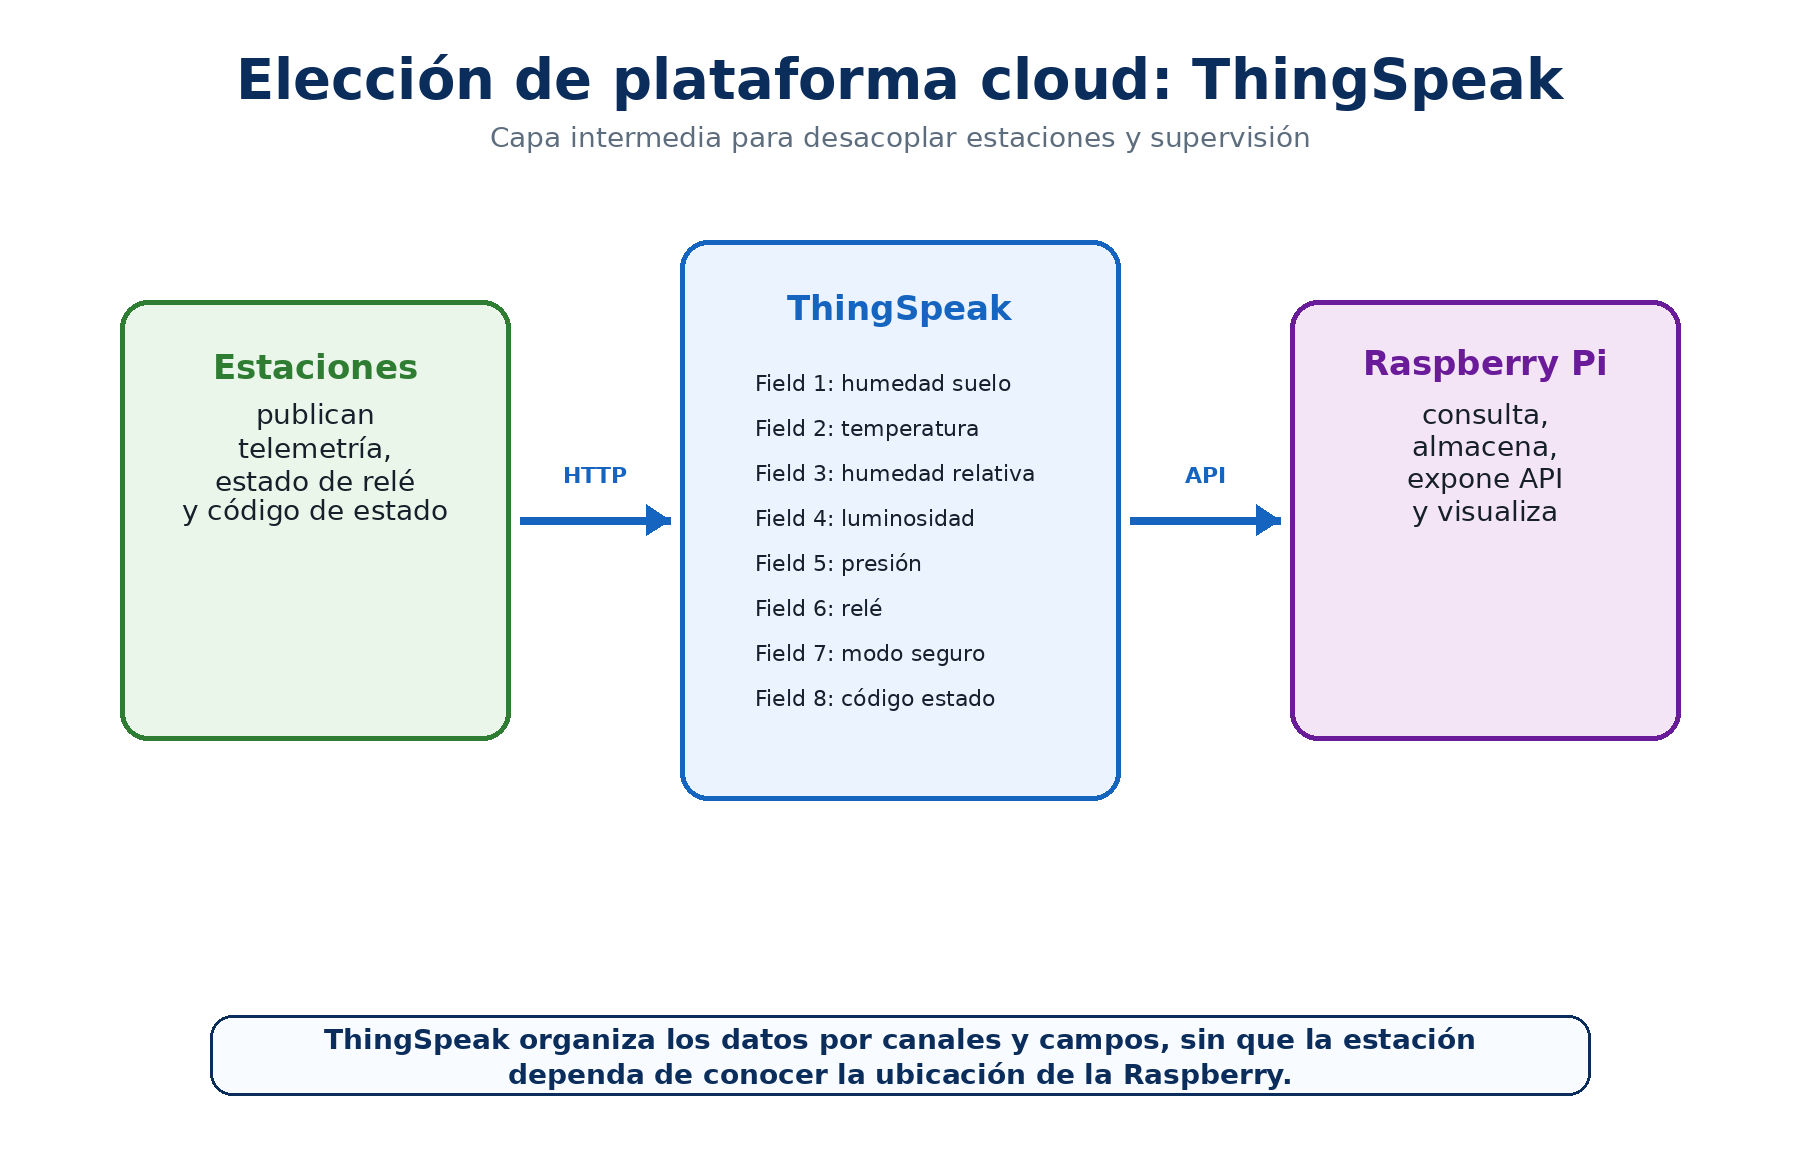
\includegraphics[width=0.78\textwidth]{figs/figura_3_9_thingspeak_capa_intermedia.png}
    \caption{Uso de ThingSpeak como capa intermedia entre estaciones remotas y sistema de supervisión. La plataforma organiza la telemetría y los estados por canales y campos, permitiendo su consulta posterior desde Raspberry Pi.}
    \label{fig:cap3_thingspeak_capa_intermedia}
\end{figure}

En TierraViva se utilizan canales diferenciados para cada estación, lo que permite separar los datos de TierraViva\_A y TierraViva\_B. Cada publicación contiene medidas ambientales, estado del relé, evento de sistema y código auxiliar de diagnóstico. Esta organización facilita la trazabilidad, evita mezclar lecturas de distintas estaciones y permite que la Raspberry Pi consulte los datos de forma independiente.

ThingSpeak presenta limitaciones que deben asumirse. No es una plataforma de tiempo real estricto y su uso introduce dependencia de conectividad, latencia y disponibilidad del servicio. Sin embargo, estas limitaciones no comprometen la actuación física del riego, ya que la decisión crítica se ejecuta localmente en cada estación. La nube se reserva para telemetría, histórico, supervisión y diagnóstico.

La estructura concreta de canales, campos y códigos publicados se desarrolla en el Capítulo~\ref{cap:capitulo4} y en el Anexo~\ref{anexo:estructura_thingspeak_estados}. La lectura de datos desde Raspberry Pi se explica en el Capítulo~\ref{cap:implementacion_software_raspberry_nube}.

\section{Elección de arquitectura software de supervisión en Raspberry Pi}
\label{sec:eleccion_arquitectura_software_raspberry}

La Raspberry Pi se ha seleccionado como sistema de supervisión software de TierraViva. Su función no es sustituir a las estaciones de campo, leer directamente los sensores ni decidir la activación de la bomba, sino consultar la información publicada por las estaciones, registrar un histórico local y ofrecer una interfaz de consulta. Esta separación resulta importante porque las estaciones se encuentran en campo y se comunican de forma remota, mientras que la Raspberry actúa como nodo de supervisión e histórico.

\begin{figure}[H]
    \centering
    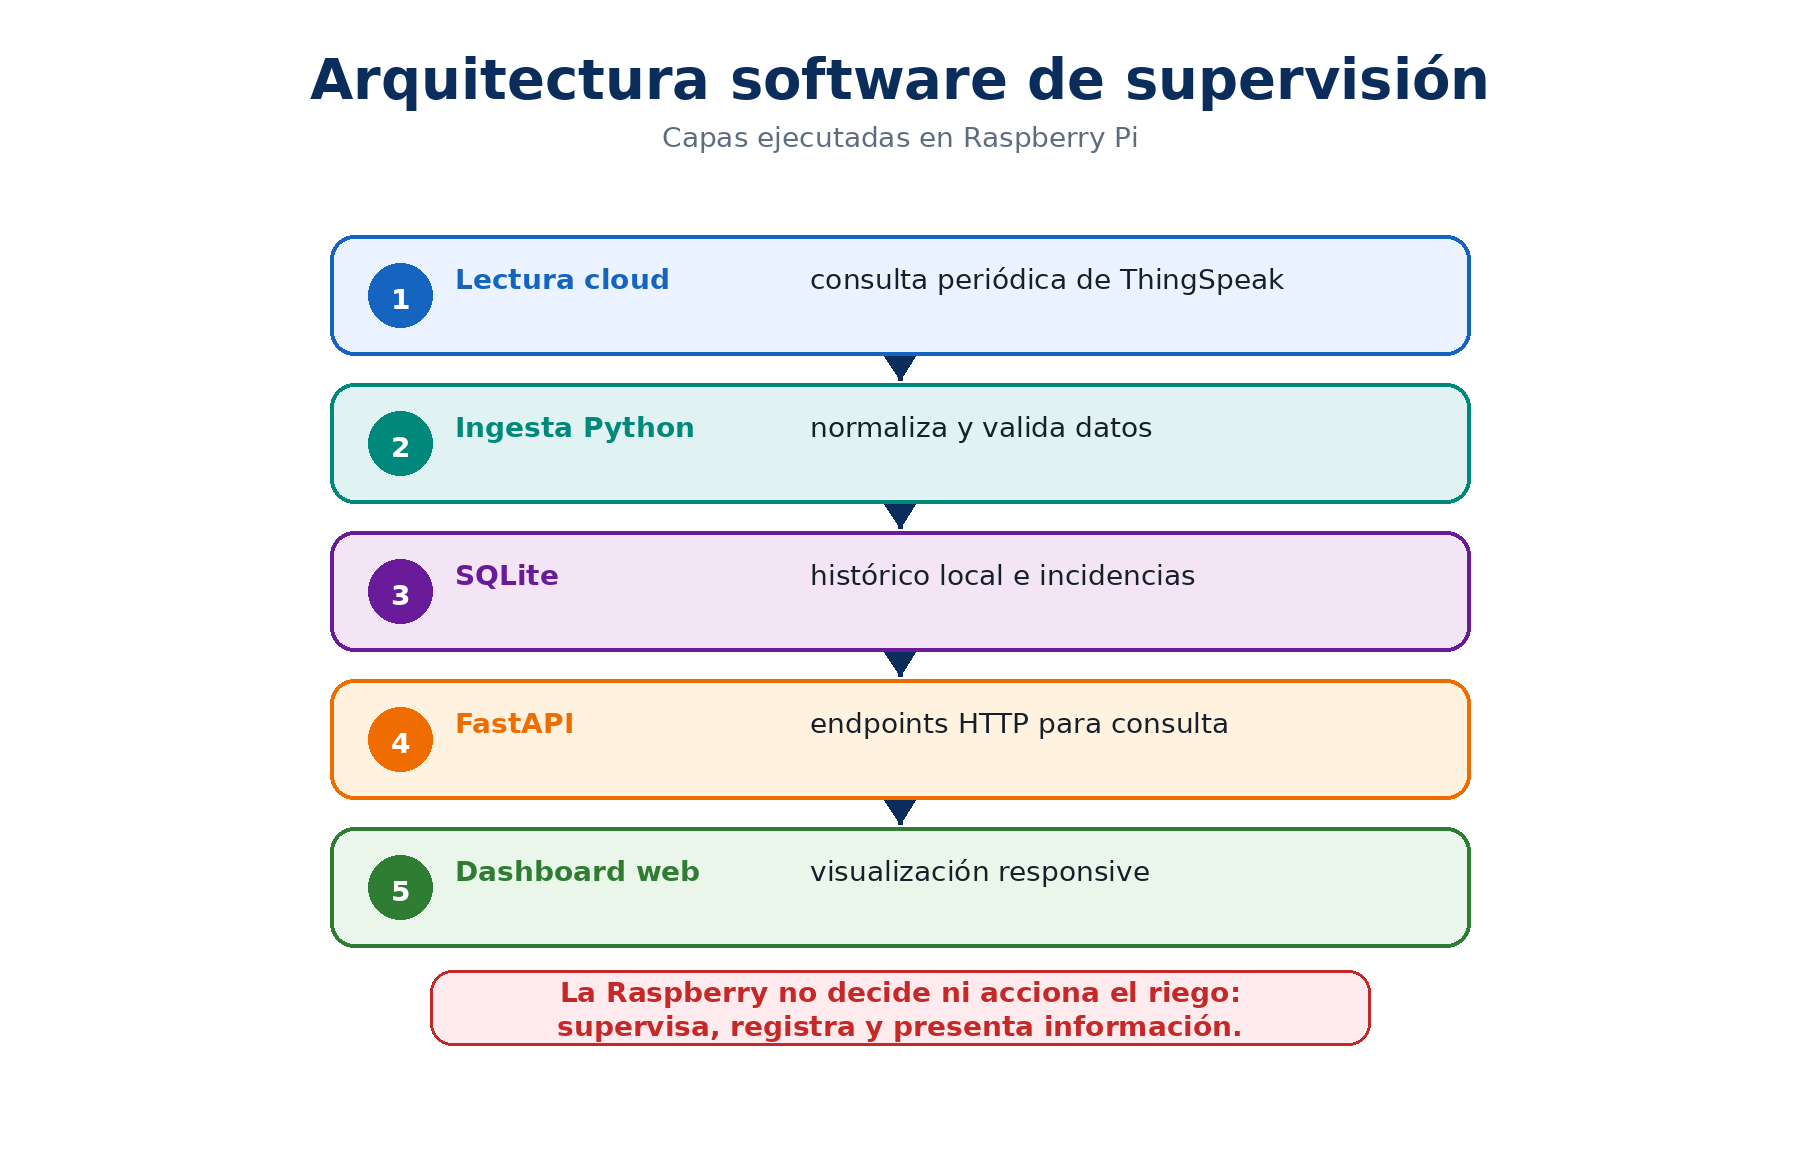
\includegraphics[width=\textwidth]{figs/figura_3_10_arquitectura_software_raspberry.png}
    \caption{Arquitectura software de supervisión en Raspberry Pi. La información publicada en la nube se consulta, valida, almacena en SQLite, expone mediante FastAPI y se presenta en el dashboard web.}
    \label{fig:cap3_arquitectura_software_raspberry}
\end{figure}

La arquitectura software de supervisión se apoya en tres bloques principales: almacenamiento local, API y dashboard. SQLite se selecciona como base de datos local por su sencillez de despliegue y por ser suficiente para conservar el histórico de lecturas, estados e incidencias del prototipo sin instalar un servidor de base de datos adicional \cite{sqlite_about}. Esta decisión permite que la Raspberry Pi mantenga una memoria propia del sistema, complementaria a los datos publicados en ThingSpeak.

FastAPI se selecciona como framework para construir la API de supervisión en Python \cite{fastapi_docs}. Su papel dentro de TierraViva es actuar como capa intermedia entre la base de datos y la interfaz web, evitando que el dashboard acceda directamente a SQLite o a los detalles internos de almacenamiento. La API permite consultar datos mediante peticiones HTTP y deja preparada la arquitectura para que otros clientes puedan reutilizar la misma información en futuras ampliaciones.

El dashboard web constituye la capa de presentación del sistema. Su objetivo es mostrar de forma comprensible las últimas lecturas, el estado de las estaciones y la información operativa publicada por cada nodo. De esta manera, la Raspberry Pi no se limita a almacenar datos, sino que los transforma en información útil para supervisar el comportamiento del prototipo.

La implementación concreta de estos bloques, incluyendo la estructura de los scripts, los endpoints expuestos, el modelo de datos y la evolución desde el prototipo local previo, se desarrolla en el Capítulo~\ref{cap:implementacion_software_raspberry_nube}.

\begin{table}[H]
\begin{center}
\small
\renewcommand{\arraystretch}{1.15}
\rowcolors{2}{TableRowSoft}{white}

\begin{tabular}{|p{0.25\textwidth}|p{0.34\textwidth}|p{0.29\textwidth}|}
\hline
\rowcolor{URJCRed}
\TVHead{Bloque software} & \TVHead{Función en TierraViva} & \TVHead{Motivo de elección} \\
\hline
Prototipo MQTT local & Validación previa de la cadena software en Raspberry. & Permitió comprobar recepción, almacenamiento, API y visualización antes de adoptar la arquitectura final con ThingSpeak. \\
\hline
Ingesta desde ThingSpeak & Consulta periódica de telemetría y estado publicados por las estaciones. & Permite alimentar el histórico local y el dashboard sin conexión directa con los nodos de campo. \\
\hline
SQLite & Almacenamiento local de lecturas, estados e incidencias. & Base de datos ligera, autocontenida y suficiente para el prototipo. \\
\hline
FastAPI & Exposición de datos mediante endpoints HTTP. & Facilita crear una API sencilla entre la base de datos y el dashboard. \\
\hline
Dashboard web & Visualización de medidas, histórico, estado del relé y estado de las estaciones. & Permite supervisar el prototipo sin acceder a consola o consultas SQL. \\
\hline
\end{tabular}
\caption{Bloques principales de la arquitectura software de supervisión en Raspberry Pi}
\label{cuadro:arquitectura_software_raspberry}
\end{center}
\end{table}

La lógica de decisión de riego no se mantiene en la Raspberry Pi en la arquitectura final. Aunque este dispositivo tiene capacidad suficiente para aplicar reglas más complejas, se ha decidido desplazar la decisión crítica al nodo de campo. Esta elección reduce la dependencia de la red y evita que la actuación física dependa de un comando remoto.

La Raspberry conserva un papel relevante como sistema de supervisión: consulta los datos publicados, mantiene un histórico local, expone la API y sirve el dashboard. La implementación concreta de estos bloques se desarrolla en el Capítulo~\ref{cap:implementacion_software_raspberry_nube}. La referencia de endpoints se recoge en el Anexo~\ref{anexo:manual_api}, y el uso de la interfaz por parte del usuario se documenta en el Anexo~\ref{anexo:manual_usuario}.

\section{Materiales empleados}
\label{sec:materiales_empleados}

La selección de materiales se ha realizado buscando un equilibrio entre funcionalidad, coste, disponibilidad y facilidad de integración. Al tratarse de un prototipo de TFG, se han utilizado módulos habituales en sistemas IoT y prototipos electrónicos, evitando componentes industriales cerrados que aumentarían el coste y dificultarían la reproducción del montaje.

Desde el punto de vista funcional, el sistema se organiza en bloques de sensórica, control local, comunicación, supervisión, actuación y alimentación. La sensórica se basa en un sensor capacitivo de humedad de suelo, BME280 y BH1750/GY-302; el control local se realiza con Arduino UNO; la comunicación remota con A7670E-LASA y tarjeta SIM; la supervisión con Raspberry Pi 5; y la actuación mediante relé y bomba de agua de 12 V.

El inventario completo, las referencias comerciales, cantidades, precios, imágenes y observaciones de compra se recogen en el Anexo~\ref{anexo:materiales}. El conexionado eléctrico se documenta en el Anexo~\ref{anexo:esquemas_electricos}, y la validación asociada a sensores, comunicación, actuación y flujo extremo a extremo se desarrolla en los Anexos~\ref{anexo:plan_pruebas} y \ref{anexo:trazabilidad_requisitos_pruebas}.

\section{Riesgos técnicos y medidas de mitigación}
\label{sec:riesgos_tecnicos_mitigacion}

El diseño de TierraViva debe contemplar fallos de sensores, alimentación, comunicación, software y actuación. Esta consideración es especialmente importante porque el prototipo no se limita a monitorizar variables ambientales, sino que acciona físicamente una bomba de agua. Por ello, el criterio general adoptado es conservador: ante una lectura inválida, una condición no verificable o un fallo relevante, la estación debe mantener la bomba apagada.

La Tabla~\ref{cuadro:riesgos_mitigacion} resume los riesgos técnicos principales considerados durante el diseño. El análisis completo de probabilidad, impacto, criticidad, riesgo residual y pruebas asociadas se desarrolla en el Anexo~\ref{anexo:gestion_riesgos}.

\begin{table}[H]
\begin{center}
\small
\renewcommand{\arraystretch}{1.15}
\rowcolors{2}{TableRowSoft}{white}

\begin{tabular}{|p{0.24\textwidth}|p{0.30\textwidth}|p{0.34\textwidth}|}
\hline
\rowcolor{URJCRed}
\TVHead{Riesgo} & \TVHead{Impacto posible} & \TVHead{Medida de mitigación} \\
\hline
Fallo de alimentación o picos de consumo & Reinicios, pérdida de comunicación o comportamiento inestable del relé. & Regulación con LM2596, comprobación de tensiones, masa común y condensadores de estabilización. \\
\hline
Lecturas erróneas o inestables & Decisiones de riego basadas en datos no fiables. & Validación de rangos, descarte de valores incoherentes, pruebas por bloques y calibración progresiva. \\
\hline
Regla local mal configurada & Activación del riego en condiciones no deseadas. & Umbrales configurables, cooldown, pruebas controladas y actuación limitada por firmware. \\
\hline
Activación prolongada de la bomba & Riego indefinido o consumo innecesario de agua. & Bomba apagada por defecto, tiempo máximo de actuación y apagado explícito al finalizar el riego. \\
\hline
Pérdida de comunicación & Ausencia de telemetría o supervisión remota incompleta. & Decisión local independiente, publicación de estados cuando sea posible y supervisión de datos obsoletos. \\
\hline
Fallo del software en Raspberry Pi & Pérdida temporal de API, dashboard o histórico local. & Separación por módulos, logs, script de gestión y autonomía de las estaciones para la decisión de riego. \\
\hline
\end{tabular}
\caption{Resumen de riesgos técnicos principales y medidas de mitigación}
\label{cuadro:riesgos_mitigacion}
\end{center}
\end{table}

Estas medidas siguen un principio común: separar supervisión y control local. La Raspberry Pi permite registrar, consultar y visualizar el estado del sistema, pero la seguridad de la actuación reside en la estación de campo. De este modo, una caída del dashboard, una pérdida de comunicación o un dato no fiable no deben provocar una activación no controlada de la bomba.

El desarrollo completo de esta gestión de riesgos se recoge en el Anexo~\ref{anexo:gestion_riesgos}. La relación entre riesgos, requisitos y pruebas se documenta además en el Anexo~\ref{anexo:trazabilidad_requisitos_pruebas}.
